\chapter{Singlet, bất đẳng thức Bell và định lý không nhân bản}

\lectureoverview{Một dấu trừ tương đối biến trạng thái hai spin chỉ tương quan đơn thuần thành trạng thái singlet bất biến đối với phép quay. Ta nhận diện trạng thái ấy bằng cách tính spin toàn phần, dùng tính phản tương quan hoàn hảo của nó để thiết lập một thí nghiệm Bell, rồi chuyển các mệnh đề cổ điển thành các toán tử chiếu lượng tử. Các xác suất thu được vi phạm bất đẳng thức đếm cổ điển của Bell. Những câu hỏi về tính địa phương, thời điểm đo và nguyên lý bất định sau đó dẫn đến một hệ quả khác của cơ học lượng tử tuyến tính: không thể sao chép một trạng thái chưa biết bằng máy nhân bản vạn năng.}

\section{Một dấu có thể tạo ra khác biệt gì?}

Xét hai electron và lược bỏ ký hiệu tích tensor trong các trạng thái cơ sở:
\begin{equation}
  \ket{ud}\equiv\ket{u}_1\otimes\ket{d}_2,
  \qquad
  \ket{du}\equiv\ket{d}_1\otimes\ket{u}_2.
\end{equation}
Hai chồng chất đặc biệt đơn giản chỉ khác nhau ở một dấu,
\begin{equation}
  \ket{\psi_\pm}
  =
  \frac{\ket{ud}\pm\ket{du}}{\sqrt2}.
  \label{eq:l05-two-signs}
\end{equation}
Thừa số \(1/\sqrt2\) bảo đảm xác suất toàn phần bằng một. Ở cả hai trạng thái, phép đo theo trục thứ ba cho hai kết quả trái ngược: nếu electron 1 có spin hướng lên thì electron 2 có spin hướng xuống, và ngược lại. Vì vậy, chỉ riêng tương quan ấy không thể phát hiện dấu này. Dẫu vậy, hai trạng thái khác nhau về mặt vật lý.

Trong các phép tính sau, ta sẽ dùng nhiều lần các tác dụng của ma trận Pauli
\begin{align}
  \sigma_1\ket{u}&=\ket{d},&
  \sigma_1\ket{d}&=\ket{u},\nonumber\\
  \sigma_2\ket{u}&=i\ket{d},&
  \sigma_2\ket{d}&=-i\ket{u},\nonumber\\
  \sigma_3\ket{u}&=\ket{u},&
  \sigma_3\ket{d}&=-\ket{d}.
  \label{eq:l05-pauli-actions}
\end{align}
Ta dùng ký hiệu \(\sigma_i\) cho các toán tử tác dụng lên electron 1 và đưa vào một họ toán tử tương tự \(\tau_i\) tác dụng lên electron 2.

\begin{figure}[htbp]
\centering
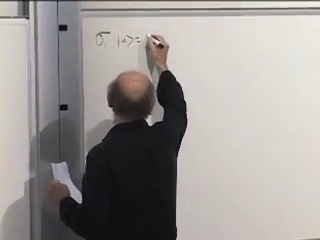
\includegraphics[width=0.62\linewidth]{lecture_05_figure_02.png}
\caption{Bảng đầy đủ về tác dụng của các ma trận Pauli được dùng xuyên suốt phần so sánh.}
\lectureframe{00:03:15}
\end{figure}

Trong cả hai trạng thái, spin của mỗi hạt cấu thành đều không có hướng ưu tiên:
\begin{equation}
  \expect{\sigma_i}_{\psi_\pm}=0,
  \qquad
  \expect{\tau_i}_{\psi_\pm}=0,
  \qquad i=1,2,3.
  \label{eq:l05-local-zero}
\end{equation}
Chẳng hạn, phép kiểm tra tường minh được yêu cầu cho trạng thái cộng cho kết quả
\begin{align}
  \bra{\psi_+}\sigma_3\ket{\psi_+}
  &=
  \frac12
  \bigl(\bra{ud}+\bra{du}\bigr)
  \bigl(\ket{ud}-\ket{du}\bigr)\nonumber\\
  &=
  \frac12(1-1)=0.
  \label{eq:l05-sigma3-expectation}
\end{align}
Các số hạng chéo triệt tiêu vì \(\braket{ud}{du}=0\).

\begin{figure}[htbp]
\centering
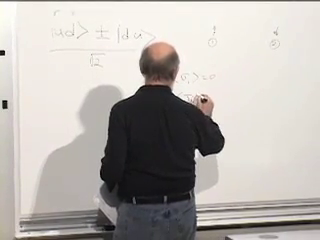
\includegraphics[width=0.78\linewidth]{lecture_05_figure_03.png}
\caption{Giá trị kỳ vọng ở trạng thái cộng được tính bằng cách cho \(\sigma_3\) tác dụng lên trạng thái rồi dùng tính trực giao.}
\lectureframe{00:07:00}
\end{figure}

\begin{classroomqa}
\lecturetimestamp{00:07:13}
\audiencequestion{Giá trị kỳ vọng bằng không có nghĩa là khi đo một spin riêng lẻ, ta có thể thu được giá trị bằng không hay không?}
\lecturerresponse{Không. Một thành phần spin chỉ có thể cho kết quả \(+1\) hoặc \(-1\); \(\sigma_i\) không có trị riêng bằng không. Phương trình~\eqref{eq:l05-local-zero} cho biết các phép đo lặp lại cho kết quả như tung đồng xu công bằng, chứ không phải mỗi lần đo đều cho kết quả bằng không.}
\end{classroomqa}

Vậy phép thử chẩn đoán đầu tiên, tuy có vẻ hợp lý, đã không thành công. Các giá trị trung bình cục bộ không thể phân biệt dấu tương đối, nên ta phải đo một đại lượng của cả cặp.

\section{Spin toàn phần chọn ra trạng thái singlet}

Mômen từ của cặp được biểu diễn bằng tổng vectơ
\begin{equation}
  \boldsymbol{\Sigma}
  =
  \boldsymbol{\sigma}+\boldsymbol{\tau}.
\end{equation}
Thành phần thứ ba của đại lượng này triệt tiêu cả hai vectơ cơ sở:
\begin{align}
  (\sigma_3+\tau_3)\ket{ud}
  &=(1-1)\ket{ud}=0,\nonumber\\
  (\sigma_3+\tau_3)\ket{du}
  &=(-1+1)\ket{du}=0.
\end{align}
Do đó,
\begin{equation}
  (\sigma_3+\tau_3)\ket{\psi_\pm}=0.
\end{equation}
Với cả hai cách chọn dấu, thành phần thứ ba của spin toàn phần đều bằng không trong mọi lần đo.

Thành phần thứ nhất phân biệt được hai trạng thái. Từ Phương trình~\eqref{eq:l05-pauli-actions},
\begin{align}
  (\sigma_1+\tau_1)\ket{ud}
  &=\ket{dd}+\ket{uu},\nonumber\\
  (\sigma_1+\tau_1)\ket{du}
  &=\ket{uu}+\ket{dd}.
\end{align}
Suy ra
\begin{align}
  (\sigma_1+\tau_1)\ket{\psi_+}
  &=
  \sqrt2\bigl(\ket{uu}+\ket{dd}\bigr),\nonumber\\
  (\sigma_1+\tau_1)\ket{\psi_-}
  &=0.
  \label{eq:l05-total-x}
\end{align}
Trạng thái cộng có thể có giá trị kỳ vọng bằng không đối với đại lượng này, nhưng nó không phải là trạng thái riêng ứng với trị riêng bằng không của đại lượng ấy.

\begin{classroomqa}
\lecturetimestamp{00:13:02}
\audiencequestion{Nếu trạng thái không bị toán tử triệt tiêu thì thành phần toàn phần có thể cho những kết quả nào?}
\lecturerresponse{Kết quả đo của mỗi hạt là \(+1\) hoặc \(-1\), nên tổng của chúng có thể là \(2\), \(0\) hoặc \(-2\). Giá trị kỳ vọng bằng không không buộc kết quả phải bằng không trong mọi lần đo.}
\end{classroomqa}

Thành phần thứ hai hoàn tất phép thử. Các thừa số \(i\) triệt tiêu nhau trong tổ hợp phản đối xứng:
\begin{equation}
  (\sigma_2+\tau_2)\ket{\psi_-}=0.
\end{equation}
Vì thế, cả ba thành phần đều triệt tiêu trạng thái trừ,
\begin{equation}
  \bigl(\boldsymbol{\sigma}+\boldsymbol{\tau}\bigr)
  \cdot\hat n\,\ket{\psi_-}=0
  \qquad\text{for every unit vector }\hat n.
  \label{eq:l05-singlet-any-axis}
\end{equation}

\begin{figure}[htbp]
\centering
\includegraphics[width=0.84\linewidth]{lecture_05_figure_06.png}
\caption{Các phép triệt tiêu theo từng thành phần xác định trạng thái trừ có spin toàn phần bằng không.}
\lectureframe{00:16:30}
\end{figure}

Trạng thái phản đối xứng \(\ket{\psi_-}\) là trạng thái \emph{singlet}. Trạng thái này bất biến đối với phép quay: đo theo trục nào cũng cho cùng một kết quả về spin toàn phần, bằng không. Trạng thái đối xứng trong Phương trình~\eqref{eq:l05-two-signs} thuộc phân hệ triplet.

\begin{classroomqa}
\lecturetimestamp{00:19:06}
\audiencequestion{Kết quả hai spin ngược chiều có đúng trong mọi lần đo hay chỉ đúng khi tính trung bình?}
\lecturerresponse{Với trạng thái singlet, điều đó đúng trong mọi lần đo. Phương trình~\eqref{eq:l05-singlet-any-axis} là một phương trình trị riêng, nên khi đo cùng một thành phần trên cả hai hạt, tổng hai kết quả luôn bằng trị riêng, tức bằng không.}
\end{classroomqa}

\begin{classroomqa}
\lecturetimestamp{00:19:36}
\audiencequestion{Vì sao trạng thái kia được gọi là triplet?}
\lecturerresponse{Tên gọi này bắt nguồn từ ba trạng thái trong đa tuyến có spin toàn phần bằng một. Ta sẽ trình bày phép suy ra sau; trong phần tính toán hiện tại, chỉ cần phân biệt trạng thái đối xứng với phân hệ singlet một chiều.}
\end{classroomqa}

Nếu Bob đo một thành phần bất kỳ của electron mình, anh ấy lập tức biết Alice sẽ thu được kết quả gì khi đo cùng thành phần trên electron của cô: kết quả của cô phải ngược lại. Đây là tương quan Einstein--Podolsky--Rosen. Một cặp đồng xu ẩn cũng có thể mang sẵn hai kết quả đối nhau, nhưng chỉ cho một câu hỏi đã được định trước. Trạng thái singlet cho tính phản tương quan hoàn hảo bất kể ta chọn trục không gian nào.

\begin{classroomqa}
\lecturetimestamp{00:20:55}
\audiencequestion{Einstein, Podolsky và Rosen có phải là những người đầu tiên phát hiện ra sự vướng víu không?}
\lecturerresponse{Không. Schrödinger đã bàn về hiện tượng này và đưa ra thuật ngữ “vướng víu”. Lập luận EPR làm nổi bật hơn vấn đề tương quan giữa các hạt ở xa nhau.}
\end{classroomqa}

\begin{classroomqa}
\lecturetimestamp{00:23:50}
\audiencequestion{Tương quan tức thời có vi phạm quan hệ nhân quả không, và việc người quan sát nào đo trước có quan trọng không?}
\lecturerresponse{Không có thông điệp hữu dụng nào được truyền đi. Dù Bob có đo hay không, kết quả đo cục bộ của Alice vẫn chia đều giữa hai khả năng trong mọi thứ tự thời gian quán tính. Cô chỉ có thể kiểm chứng tương quan sau khi nhận kết quả của Bob qua một kênh cổ điển thông thường, vốn không thể truyền nhanh hơn ánh sáng.}
\end{classroomqa}

\section{Bất đẳng thức Bell là phép đếm cổ điển}

Ta có thể cảm nhận kết quả của Bell theo những cách không thống nhất. Có lúc nó dường như là đặc điểm sâu sắc nhất của cơ học lượng tử; lúc khác, nó lại có vẻ là một hệ quả tất yếu nữa của hình thức luận. Bản thân Bell và cả Feynman đều có thể bày tỏ cả hai cách nhìn. Tuy nhiên, bất đẳng thức này rất sơ đẳng. Điều đáng ngạc nhiên là nó bị vi phạm.

Xét một tập hợp vật thể thông thường. Mỗi vật thể có thể có hoặc không có ba tính chất \(A\), \(B\) và \(C\). Gọi \(N(A,\neg B)\) là số vật thể có \(A\) nhưng không có \(B\). Lôgic tập hợp cổ điển cho ta
\begin{equation}
  N(A,\neg B)+N(B,\neg C)
  \geq
  N(A,\neg C).
  \label{eq:l05-bell-count}
\end{equation}
Chứng minh dựa trên phép bao hàm tập hợp
\begin{equation}
  A\cap C^{c}
  \subseteq
  (A\cap B^{c})\cup(B\cap C^{c}).
  \label{eq:l05-set-inclusion}
\end{equation}
Thật vậy, một phần tử thuộc \(A\cap C^c\) hoặc thuộc \(B\), hoặc không thuộc tập hợp đó. Trong trường hợp thứ nhất, phần tử ấy thuộc \(B\cap C^c\); trong trường hợp thứ hai, nó thuộc \(A\cap B^c\). Đếm hợp của hai tập chỉ có thể cho số lượng lớn hơn hoặc bằng số phần tử của tập ở vế trái.

\begin{figure}[htbp]
\centering
\includegraphics[width=0.78\linewidth]{lecture_05_figure_07.png}
\caption{Chứng minh trên bảng chia ba tập con cổ điển có phần giao nhau thành các miền không âm.}
\lectureframe{00:31:15}
\end{figure}

Tương đương, hãy gán cho các miền rời nhau trong sơ đồ ba tập những số nguyên không âm \(N_i\). Cả hai vế của Phương trình~\eqref{eq:l05-bell-count} đều bao gồm các miền thuộc \(A\cap C^c\), trong khi vế trái còn bao gồm thêm những miền không âm khác. Ở đây chưa có yếu tố lượng tử nào. Đây là một định lý về các tập con và những khả năng lôgic thông thường.

\section{Chuyển mệnh đề tập hợp thành thí nghiệm spin}

Chuẩn bị nhiều cặp electron độc lập ở trạng thái singlet và xác định ba mệnh đề về electron 1:
\begin{align}
  A&:\ \text{spin 1 is up at }0^\circ\text{, along the third axis},\nonumber\\
  B&:\ \text{spin 1 is up at }45^\circ\text{ in the }zx\text{-plane},\nonumber\\
  C&:\ \text{spin 1 is up at }90^\circ\text{, along the first axis}.
  \label{eq:l05-abc}
\end{align}

\begin{figure}[htbp]
\centering
\includegraphics[width=0.82\linewidth]{lecture_05_figure_08.png}
\caption{Ba mệnh đề spin được cố định tại các góc \(0^\circ\), \(45^\circ\) và \(90^\circ\) trong cùng một mặt phẳng.}
\lectureframe{00:39:00}
\end{figure}

Trong trạng thái singlet, phủ định của một mệnh đề về electron 1 có thể được viết lại thành một mệnh đề khẳng định về electron 2. Chẳng hạn,
\begin{align}
  \neg B
  &:\ \text{spin 1 is down at }45^\circ\nonumber\\
  &\Longleftrightarrow
  \text{spin 2 is up at }45^\circ.
\end{align}
Tương tự, \(\neg C\) trở thành mệnh đề rằng electron 2 có spin hướng lên tại \(90^\circ\).

\begin{classroomqa}
\lecturetimestamp{00:40:04}
\audiencequestion{Có phải \(\neg C\) khiến electron 2 có spin hướng xuống tại \(90^\circ\) không?}
\lecturerresponse{Không. Trước hết, phủ định \(C\): electron 1 có spin hướng xuống tại \(90^\circ\). Tính phản tương quan hoàn hảo của trạng thái singlet sau đó cho biết electron 2 có spin hướng lên theo cùng trục ấy. Phải tách riêng hai lần đảo chiều này.}
\end{classroomqa}

Với một tập hợp lớn, số đếm và xác suất chỉ khác nhau bởi cùng một hệ số là số cặp đã chuẩn bị. Tính bất biến quay cũng cho
\begin{equation}
  P(A,\neg B)=P(B,\neg C),
\end{equation}
bởi vì thí nghiệm thứ hai là thí nghiệm thứ nhất sau khi quay đi một góc \(45^\circ\). Vì vậy, bất đẳng thức cổ điển của Bell đòi hỏi
\begin{equation}
  2P(A,\neg B)\geq P(A,\neg C).
  \label{eq:l05-bell-probability}
\end{equation}
Giờ ta cần một cách hiệu quả để tính các xác suất này.

\section{Mệnh đề trở thành toán tử chiếu}

Trong không gian vectơ ba chiều thông thường, toán tử chiếu loại bỏ mọi thành phần vuông góc với một không gian con đã chọn. Toán tử chiếu một chiều chiếu trực giao vectơ lên một đường thẳng; toán tử chiếu hai chiều chiếu nó lên một mặt phẳng. Nếu \(P\) chiếu lên một không gian con xác định thì
\begin{equation}
  P\ket{\alpha}=\ket{\alpha_P}.
\end{equation}

\begin{figure}[htbp]
\centering
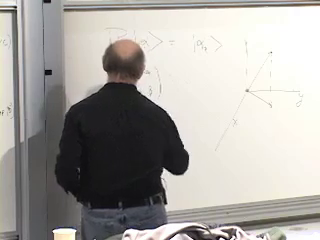
\includegraphics[width=0.76\linewidth]{lecture_05_figure_04.png}
\caption{Phép chiếu hình học và ký hiệu toán tử được trình bày song song.}
\lectureframe{00:49:53}
\end{figure}

\begin{figure}[htbp]
\centering
\begin{tikzpicture}[scale=1.05,>=Latex]
  \draw[->] (-0.25,0)--(4.0,0);
  \draw[thick] (-0.25,-0.25)--(3.55,2.6);
  \draw[->,very thick] (0,0)--(2.25,3.05)
    node[above] {\(\ket{\alpha}\)};
  \coordinate (P) at (2.72,1.98);
  \draw[dashed] (2.25,3.05)--(P);
  \draw[->,very thick] (0,0)--(P)
    node[right] {\(\ket{\alpha_P}\)};
  \node[below right] at (3.1,2.25) {projected subspace};
\end{tikzpicture}
\caption{Dựng lại hình học phép chiếu một cách rõ ràng.}
\end{figure}

Trong không gian Hilbert của một spin, mệnh đề \(\sigma_3=+1\) tương ứng với không gian con một chiều được sinh bởi \(\ket{u}\). Toán tử chiếu của nó tác dụng như sau:
\begin{equation}
  P_{\sigma_3=+1}
  \begin{pmatrix}\alpha\\\beta\end{pmatrix}
  =
  \begin{pmatrix}\alpha\\0\end{pmatrix},
  \qquad
  P_{\sigma_3=-1}
  \begin{pmatrix}\alpha\\\beta\end{pmatrix}
  =
  \begin{pmatrix}0\\\beta\end{pmatrix}.
  \label{eq:l05-projector-actions}
\end{equation}

\begin{classroomqa}
\lecturetimestamp{00:49:55}
\audiencequestion{Toán tử chiếu thứ nhất có cho biết vectơ vươn cao đến đâu trên trục thẳng đứng không?}
\lecturerresponse{Không. Nó chỉ loại bỏ hệ số trực giao \(\beta\). Các thành phần ở đây là biên độ trong không gian Hilbert, chứ không phải tọa độ không gian thông thường của spin.}
\end{classroomqa}

\begin{figure}[htbp]
\centering
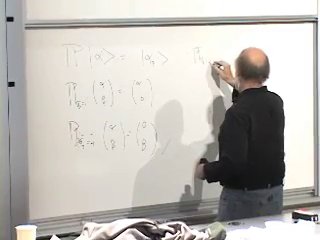
\includegraphics[width=0.78\linewidth]{lecture_05_figure_05.png}
\caption{Trước hết, toán tử chiếu tác dụng lên một spinor tổng quát, sau đó được viết dưới dạng ma trận tường minh.}
\lectureframe{00:51:40}
\end{figure}

Dạng ma trận là
\begin{equation}
  P_{\sigma_3=+1}
  =
  \begin{pmatrix}1&0\\0&0\end{pmatrix}
  =
  \frac{I+\sigma_3}{2}.
  \label{eq:l05-p3}
\end{equation}
Phép dựng tương tự áp dụng cho một vectơ đơn vị bất kỳ \(\hat n\):
\begin{equation}
  P_{\boldsymbol{\sigma}\cdot\hat n=+1}
  =
  \frac{I+\boldsymbol{\sigma}\cdot\hat n}{2}.
  \label{eq:l05-pn}
\end{equation}

\begin{classroomqa}
\lecturetimestamp{00:53:09}
\audiencequestion{Toán tử chiếu lên \(\sigma_1=+1\) là gì?}
\lecturerresponse{Trong Phương trình~\eqref{eq:l05-p3}, thay \(\sigma_3\) bằng \(\sigma_1\): \(P_{\sigma_1=+1}=(I+\sigma_1)/2\).}
\end{classroomqa}

Giờ đây, quy tắc Born có thể được viết dưới dạng mệnh đề hữu ích:
\begin{equation}
  P(\mathcal A\text{ is true in }\ket{\psi})
  =
  \bra{\psi}P_{\mathcal A}\ket{\psi}.
  \label{eq:l05-projector-born}
\end{equation}
Với spinor đã chuẩn hóa \(\ket{\psi}=(\alpha,\beta)^T\), Phương trình~\eqref{eq:l05-projector-born} khi \(P_{\sigma_3=+1}\) cho kết quả \(|\alpha|^2\), đúng như mong đợi.

Cách diễn đạt này cho thấy sự khác biệt giữa mệnh đề cổ điển và mệnh đề lượng tử. Trong lôgic cổ điển, một tính chất tương ứng với một tập con của một tập hợp. Trong cơ học lượng tử, một tính chất tương ứng với một không gian con của không gian Hilbert, hay tương đương với toán tử chiếu lên không gian đó. Các phép toán trên tập con và trên không gian con vectơ không tuân theo cùng một cấu trúc lưới; mâu thuẫn của Bell bắt nguồn từ sự khác biệt ấy.

\subsection{Toán tử chiếu Bell đồng thời}

Để \(A\wedge\neg B\), electron 1 phải có spin hướng lên theo trục thứ ba, còn electron 2 phải có spin hướng lên theo trục
\begin{equation}
  \hat n_{45}=\frac{\hat x+\hat z}{\sqrt2}.
\end{equation}
Thành phần thích hợp của spin thứ hai là
\begin{equation}
  \boldsymbol{\tau}\cdot\hat n_{45}
  =
  \frac{\tau_1+\tau_3}{\sqrt2}.
\end{equation}
Vì vậy, toán tử chiếu đồng thời là
\begin{equation}
  P_{A\wedge\neg B}
  =
  \frac{I+\sigma_3}{2}
  \frac{I+(\tau_1+\tau_3)/\sqrt2}{2}.
  \label{eq:l05-joint-projector}
\end{equation}

\begin{classroomqa}
\lecturetimestamp{00:59:18}
\audiencequestion{Vì sao thành phần spin theo hướng \(45^\circ\) có thừa số \(1/\sqrt2\)?}
\lecturerresponse{Vectơ chỉ phương phải là vectơ đơn vị. Các thành phần theo trục thứ nhất và trục thứ ba đều bằng \(1/\sqrt2\), nên đại lượng quan sát tương ứng là \((\tau_1+\tau_3)/\sqrt2\).}
\end{classroomqa}

\begin{classroomqa}
\lecturetimestamp{01:00:52}
\audiencequestion{Toàn bộ biểu thức \(I+\boldsymbol{\tau}\cdot\hat n_{45}\) có được chia cho hai không?}
\lecturerresponse{Đúng. Toán tử chiếu là \(\bigl(I+\boldsymbol{\tau}\cdot\hat n_{45}\bigr)/2\); thừa số \(1/2\) nhân với toàn bộ tử số.}
\end{classroomqa}

Hai thừa số trong Phương trình~\eqref{eq:l05-joint-projector} tác dụng lên hai thừa số tensor khác nhau nên giao hoán. Tác dụng cả hai trước hết loại bỏ mọi thành phần mà electron 1 có spin hướng xuống, rồi loại bỏ mọi thành phần còn lại mà electron 2 có spin hướng xuống theo \(\hat n_{45}\).

\section{Các số lượng tử đảo ngược bất đẳng thức}

Gọi
\begin{equation}
  \ket{\psi_s}
  =
  \frac{\ket{ud}-\ket{du}}{\sqrt2}
\end{equation}
là trạng thái singlet. Bắt đầu với
\begin{equation}
  P(A,\neg B)
  =
  \bra{\psi_s}P_{A\wedge\neg B}\ket{\psi_s}.
\end{equation}
Thừa số \((I+\sigma_3)/2\) triệt tiêu \(\ket{du}\) và giữ lại \(\ket{ud}/\sqrt2\). Tiếp đó, thừa số thứ hai cho
\begin{align}
  \frac{I+(\tau_1+\tau_3)/\sqrt2}{2}\ket{ud}
  &\notag\\[-0.3em]
  &=
  \frac12
  \left[
    \ket{ud}
    +\frac{\ket{uu}-\ket{ud}}{\sqrt2}
  \right]\nonumber\\
  &=
  \frac12
  \Biggl[
    \left(1-\frac1{\sqrt2}\right)\ket{ud}
  \nonumber\\
  &\qquad
    +\frac1{\sqrt2}\ket{uu}\Biggr].
  \label{eq:l05-projector-action}
\end{align}
Số hạng \(\ket{uu}\) có tích vô hướng với bra singlet bằng không, còn các thừa số chuẩn hóa còn lại cho
\begin{equation}
  P(A,\neg B)
  =
  \frac14\left(1-\frac1{\sqrt2}\right).
  \label{eq:l05-pab}
\end{equation}

\begin{figure}[htbp]
\centering
\includegraphics[width=0.88\linewidth]{lecture_05_figure_09.png}
\caption{Phép tính với toán tử chiếu giữ lại thành phần chiếu \(\ket{ud}\) và loại bỏ thành phần trực giao \(\ket{uu}\).}
\lectureframe{01:08:20}
\end{figure}

Tính bất biến quay cho cùng kết quả với cặp hướng tiếp theo:
\begin{equation}
  P(B,\neg C)
  =
  \frac14\left(1-\frac1{\sqrt2}\right).
\end{equation}
Với \(A\wedge\neg C\), trục thứ hai trùng với trục không gian thứ nhất, nên
\begin{equation}
  P_{A\wedge\neg C}
  =
  \frac{I+\sigma_3}{2}\frac{I+\tau_1}{2}.
\end{equation}
Thừa số thứ nhất một lần nữa giữ lại \(\ket{ud}/\sqrt2\). Số hạng \(\tau_1\) tạo ra \(\ket{uu}\), trực giao với bra singlet, trong khi số hạng đơn vị được giữ lại. Do đó,
\begin{equation}
  P(A,\neg C)=\frac14.
  \label{eq:l05-pac}
\end{equation}
Kết hợp ba kết quả,
\begin{equation}
  \underbrace{
  P(A,\neg B)+P(B,\neg C)
  }_{\frac12(1-1/\sqrt2)\approx0.146}
  <
  \underbrace{
  P(A,\neg C)
  }_{\frac14=0.25}.
  \label{eq:l05-bell-violation}
\end{equation}

\begin{figure}[htbp]
\centering
\includegraphics[width=0.84\linewidth]{lecture_05_figure_10.png}
\caption{Phép tính hoàn chỉnh trên bảng cho thấy vế trái của bất đẳng thức Bell nhỏ hơn vế phải.}
\lectureframe{01:12:15}
\end{figure}

Phương trình~\eqref{eq:l05-bell-violation} đảo ngược Phương trình~\eqref{eq:l05-bell-probability}. Kết luận không phải là cơ học lượng tử tự mâu thuẫn. Kết luận là các tương quan của trạng thái singlet không thể phát sinh từ một mô hình cổ điển địa phương, trong đó cả ba mệnh đề spin đều có giá trị chân lý theo lý thuyết tập hợp thông thường, độc lập với lựa chọn phép đo ở xa. Một mô phỏng cổ điển chỉ có thể tái tạo các tương quan ấy nếu từ bỏ ít nhất một giả định của Bell, rõ rệt nhất là tính địa phương.

\section{Thí nghiệm Bell kiểm tra điều gì}

Cơ học lượng tử đã dự đoán sự vi phạm này. Thí nghiệm còn phải loại trừ khả năng thoát khỏi kết luận cổ điển, theo đó một máy dò báo cho máy dò kia biết nó gặp thiết lập hay kết quả nào. Hai nhánh thí nghiệm cần cách nhau đủ xa, còn các lựa chọn và phép phát hiện phải đủ gần nhau về thời gian, sao cho tín hiệu truyền với tốc độ ánh sáng không thể đi từ nhánh này sang nhánh kia. Thí nghiệm của Aspect khiến yêu cầu về thời điểm và sự cô lập trở nên thuyết phục trên phương diện thực nghiệm.

\begin{classroomqa}
\lecturetimestamp{01:13:15}
\audiencequestion{Nếu cơ học lượng tử đã cho sẵn đáp án, các thí nghiệm Bell giúp ta biết thêm điều gì?}
\lecturerresponse{Chúng kiểm tra xem tự nhiên có tuân theo dự đoán lượng tử trong chính thí nghiệm tương quan này hay không; điều cốt yếu là chúng khiến hai nhánh đo độc lập với nhau trong khoảng thời gian ánh sáng truyền giữa chúng. Việc kiểm soát thí nghiệm và thời điểm đo tự thân đã là những thành tựu đáng kể.}
\end{classroomqa}

\begin{classroomqa}
\lecturetimestamp{01:18:19}
\audiencequestion{Bell đã bổ sung điều gì sau khi Einstein bàn về tác động ma quái?}
\lecturerresponse{Bell đưa ra một bất đẳng thức định lượng. Ông chỉ ra một thí nghiệm tương quan khả thi mà dự đoán lượng tử của nó loại trừ cách giải thích nền tảng cổ điển địa phương, thay vì chỉ dừng lại ở cảm giác bất an về mặt triết học. Bell vẫn phân vân liệu điều này là tất yếu hay sâu sắc, và ngày càng sẵn lòng chất vấn cơ học lượng tử chuẩn.}
\end{classroomqa}

Các hạt có thể cách xa nhau hàng dặm mà vẫn cùng thuộc về một trạng thái chung, nhưng đây vẫn là một thí nghiệm lượng tử trên các hệ nhỏ. Tương tác với môi trường có xu hướng phá hủy những quan hệ pha cần thiết. Các phân tử không khí, photon lạc và nhiễu động nhiệt có thể vướng víu với cặp hạt, vì vậy cần thực hiện thí nghiệm trong môi trường lạnh và cách ly tốt.

\begin{classroomqa}
\lecturetimestamp{01:19:53}
\audiencequestion{Một trạng thái chung trải rộng trên khoảng cách lớn có khiến đây trở thành vật thể lượng tử vĩ mô không?}
\lecturerresponse{Mô tả phù hợp hơn là các hệ lượng tử nhỏ ở cách xa nhau. Khoảng cách giữa chúng có thể lớn, nhưng việc bảo toàn hàm sóng chung ngày càng mong manh vì tương tác không kiểm soát được với môi trường phá hủy độ kết hợp hữu ích. Hai quả bóng bowling thông thường không tạo nên thí nghiệm tương tự.}
\end{classroomqa}

\begin{classroomqa}
\lecturetimestamp{01:21:23}
\audiencequestion{Đo một hạt có thể cho biết thông tin bổ sung về hạt kia, qua đó lách nguyên lý bất định hay không?}
\lecturerresponse{Ta có thể đo chẳng hạn vị trí của hạt này và động lượng của hạt kia. Đó không phải là phép đo đồng thời các đại lượng không giao hoán trên cùng một hạt. Hạn chế bất định đối với một hệ đơn lẻ vẫn không bị lách qua.}
\end{classroomqa}

\section{Khi nào tích có nghĩa là “và”?}

Trong phép tính Bell, ta nhân hai toán tử chiếu. Tích này chỉ biểu diễn phép hội khi hai mệnh đề tương thích.

\begin{classroomqa}
\lecturetimestamp{01:22:39}
\audiencequestion{Vì sao tích của hai toán tử chiếu biểu diễn từ lôgic “và”?}
\lecturerresponse{Vì hai toán tử chiếu giao hoán. Một toán tử tác dụng lên electron 1, toán tử kia tác dụng lên electron 2, nên thứ tự không quan trọng và có thể kiểm tra đồng thời cả hai tính chất. Với một electron duy nhất, \((I+\sigma_3)/2\) và \((I+\sigma_1)/2\) không giao hoán; spin hướng lên theo cả hai trục không phải là một mệnh đề đồng thời xác định theo nghĩa này.}
\end{classroomqa}

Đây là một điểm khác nữa cho thấy các mệnh đề lượng tử khác với các tập con thông thường. Giao của hai tập cổ điển luôn xác định được. Vật tương tự trong cơ học lượng tử, được biểu diễn bằng tích các toán tử chiếu, chỉ mang ý nghĩa lôgic dự định khi các không gian con liên quan tương thích.

Cùng mạch thảo luận này cũng dẫn đến vấn đề phép đo. Thiết bị đo có trạng thái kim chỉ. Nếu electron spin hướng lên làm kim lệch theo một hướng còn electron spin hướng xuống làm kim lệch theo hướng kia, thì electron ở trạng thái chồng chất sẽ vướng víu với hai vị trí kim. Vì vậy, có thể nghiên cứu phép đo như sự vướng víu giữa hệ và thiết bị. Ta sẽ gác vấn đề đó lại và xét một định lý ngắn hơn, chỉ cần dùng tính tuyến tính.

\begin{classroomqa}
\lecturetimestamp{01:25:09}
\audiencequestion{Có thể xem sự sụp đổ hàm sóng một cách hữu ích như một phép đo ràng buộc trạng thái chung hay không?}
\lecturerresponse{Câu hỏi đó thuộc về quá trình đo. Thiết bị và hệ được đo trở nên vướng víu: một giá trị spin tương quan với một vị trí kim, còn giá trị kia tương quan với vị trí khác. Ta sẽ bàn chi tiết về phép đo sau.}
\end{classroomqa}

\section{Tính tuyến tính cấm máy photocopy vạn năng}

Chỉ cần biết một điều về sự tiến hóa theo thời gian. Nếu một quá trình vật lý biến đổi
\begin{equation}
  \ket{a}\longrightarrow\ket{a'},
  \qquad
  \ket{b}\longrightarrow\ket{b'},
\end{equation}
thì tính tuyến tính đòi hỏi
\begin{equation}
  \alpha\ket{a}+\beta\ket{b}
  \longrightarrow
  \alpha\ket{a'}+\beta\ket{b'}.
  \label{eq:l05-linearity}
\end{equation}

Máy photocopy thông thường có thể tái tạo thông tin cổ điển với sai số nhỏ đến mức có thể kiểm soát. Yêu cầu lượng tử mạnh hơn: một thiết bị cố định phải sao chép đầy đủ mọi biên độ của bất kỳ trạng thái nào được đưa vào. Vì vậy, định lý không nhân bản còn được gọi là nguyên lý không thể photocopy lượng tử.

Hãy hình dung một máy có một cổng vào và hai cổng ra. Nếu máy nhân bản được các trạng thái cơ sở theo trục thứ ba, nó phải thực hiện
\begin{equation}
  \ket{u}\longrightarrow\ket{uu},
  \qquad
  \ket{d}\longrightarrow\ket{dd}.
  \label{eq:l05-clone-basis}
\end{equation}
Máy có thể cung cấp năng lượng, khối lượng hoặc điện tích cho các đầu ra; việc hạch toán bảo toàn không phải là trở ngại. Mâu thuẫn nằm ở sự phụ thuộc của phép biến đổi vào trạng thái.

\begin{figure}[H]
\centering
\includegraphics[width=0.86\linewidth]{lecture_05_figure_11.png}
\caption{Một máy giả định có một đầu vào và hai đầu ra được yêu cầu sao chép cả hai trạng thái cơ sở.}
\lectureframe{01:33:45}
\end{figure}

Giờ hãy đưa vào một spin hướng sang phải,
\begin{equation}
  \ket{r}
  =
  \frac{\ket{u}+\ket{d}}{\sqrt2}.
  \label{eq:l05-right-state}
\end{equation}
Các Phương trình~\eqref{eq:l05-linearity} và \eqref{eq:l05-clone-basis} buộc đầu ra phải là
\begin{equation}
  \ket{r}
  \longrightarrow
  \frac{\ket{uu}+\ket{dd}}{\sqrt2}.
  \label{eq:l05-linear-output}
\end{equation}
Trong khi đó, phép nhân bản chính xác đòi hỏi hai bản sao độc lập:
\begin{align}
  \ket{rr}
  &=
  \ket{r}\otimes\ket{r}\nonumber\\
  &=
  \frac12
  \left(
    \ket{uu}+\ket{ud}+\ket{du}+\ket{dd}
  \right).
  \label{eq:l05-cloned-output}
\end{align}
Các số hạng hỗn hợp có trong Phương trình~\eqref{eq:l05-cloned-output} lại vắng mặt trong Phương trình~\eqref{eq:l05-linear-output}. Hai đầu ra khác nhau.

\begin{figure}[H]
\centering
\includegraphics[width=0.72\linewidth]{lecture_05_figure_12.png}
\caption{Tính tuyến tính chỉ tạo ra các số hạng có spin song song, trong khi hai bản sao thực sự của trạng thái hướng sang phải còn có cả hai số hạng hỗn hợp.}
\lectureframe{01:35:20}
\end{figure}

\begin{theorem}[No-cloning]
Không một máy vật lý nào có thể nhân bản chính xác mọi trạng thái lượng tử chưa biết.
\end{theorem}

\begin{proof}
Giả sử một máy nhân bản các trạng thái cơ sở trực giao như trong Phương trình~\eqref{eq:l05-clone-basis}. Tính tuyến tính khi đó xác định đầu ra của máy đối với chồng chất của chúng là Phương trình~\eqref{eq:l05-linear-output}. Nhân bản chính xác cùng trạng thái đầu vào đòi hỏi Phương trình~\eqref{eq:l05-cloned-output}. Vì hai vectơ trạng thái này khác nhau nên máy vạn năng giả định không thể tồn tại.
\end{proof}

Lý do nằm ở cấu trúc. Phép biến đổi \(\ket{\psi}\) thành \(\ket{\psi}\otimes\ket{\psi}\) là bậc hai theo các biên độ, trong khi mọi sự tiến hóa được phép của trạng thái lượng tử toàn phần đều tuyến tính.

\begin{classroomqa}
\lecturetimestamp{01:35:49}
\audiencequestion{Chứng minh này có giả định hai đầu ra độc lập không?}
\lecturerresponse{Có, bởi vì hai bản sao phải là các bản sao độc lập có thể sử dụng riêng. Các hệ độc lập kết hợp với nhau bằng tích tensor, vì thế hai bản sao hướng sang phải là \(\ket{r}\otimes\ket{r}\). Đầu ra có tương quan nhưng không thể sử dụng riêng không phải là hai bản sao.}
\end{classroomqa}

\begin{classroomqa}
\lecturetimestamp{01:37:20}
\audiencequestion{Laser dường như sao chép trạng thái photon thông qua phát xạ kích thích. Lập luận trên sai ở đâu?}
\lecturerresponse{Nguyên tử và các mode điện từ cũng tham gia vào quá trình. Trạng thái của chúng góp phần tạo nên đầu ra và biểu hiện thành nhiễu khi xét bài toán nhân bản vạn năng. Có thể nhân bản gần đúng, nhưng không thể nhân bản hoàn hảo mà không phụ thuộc vào trạng thái.}
\end{classroomqa}

\begin{classroomqa}
\lecturetimestamp{01:40:24}
\audiencequestion{Có thể truyền thông tin lượng tử dù không thể nhân bản nó không?}
\lecturerresponse{Có. Truyền là một phép biến đổi khác: không cần giữ trạng thái ở vật mang ban đầu. Định lý không nhân bản cấm kết thúc quá trình với hai bản sao hoàn hảo độc lập, chứ không cấm chuyển trạng thái từ vật mang này sang vật mang khác.}
\end{classroomqa}

\begin{classroomqa}
\lecturetimestamp{01:41:03}
\audiencequestion{Trạng thái đầu vào có nhất thiết phải chưa biết không?}
\lecturerresponse{Nếu biết trước trạng thái, ta có thể chuẩn bị thêm các hệ ở trạng thái đó, hoặc chế tạo thiết bị thích ứng với một cơ sở trực giao đã chọn. Điều không thể làm là dùng một máy nhận đầu vào tùy ý và nhân bản nó mà không biết trước trạng thái nào đã được đưa vào.}
\end{classroomqa}

\begin{classroomqa}
\lecturetimestamp{01:42:35}
\audiencequestion{Trong hai biểu thức trạng thái hướng sang phải, biểu thức nào là đầu ra thực sự của máy?}
\lecturerresponse{Tính tuyến tính buộc đầu ra phải theo Phương trình~\eqref{eq:l05-linear-output}; còn việc nhân bản đòi hỏi Phương trình~\eqref{eq:l05-cloned-output}. Sự bất đồng giữa hai biểu thức chính là mâu thuẫn.}
\end{classroomqa}

\begin{classroomqa}
\lecturetimestamp{01:43:40}
\audiencequestion{Có thể định lượng lượng thông tin bổ sung mà trạng thái vướng víu hai hạt mang theo không?}
\lecturerresponse{Một trạng thái thuần của một spin có hai tham số vật lý thực. Hai spin được chuẩn bị riêng biệt có tổng cộng bốn tham số, trong khi một trạng thái thuần tổng quát trong không gian Hilbert bốn chiều của hai spin có sáu tham số sau khi bỏ chuẩn hóa và pha toàn cục. Các trạng thái bổ sung bao gồm trạng thái vướng víu; mức độ vướng víu của chúng có thể được định lượng bằng entropy vướng víu.}
\end{classroomqa}

\enlargethispage{4\baselineskip}
Dấu trong Phương trình~\eqref{eq:l05-two-signs} vừa đảm nhiệm ba vai trò. Nó chọn ra trạng thái duy nhất có spin toàn phần bằng không, tạo nên các tương quan vi phạm bất đẳng thức tập hợp cổ điển, và làm lộ rõ khác biệt giữa sự tiến hóa lượng tử tuyến tính với thao tác phi tuyến tạo ra hai bản sao. Mỗi kết quả đều bắt nguồn từ việc xem trạng thái chung là một vectơ trong toàn bộ không gian tích tensor, thay vì một danh sách các tính chất cục bộ có sẵn.
